% Submission LaTeX for SoftwareX (simplified)
\documentclass[11pt]{article}
\usepackage{graphicx}
\usepackage{authblk}
\usepackage{hyperref}
\title{PiXY: Pixel to stage-XY Coordinate Converter}
\author[1]{Yoshiaki KON}
\affil[1]{Geological Survey of Japan (GSJ), National Institute of Advanced Industrial Science and Technology (AIST)}
\date{29 January 2026}
\begin{document}
\maketitle
\begin{abstract}
PiXY is an open-source GUI tool that converts pixel coordinates from microscopy images into instrument stage coordinates to speed micrometer-scale targeting in in-situ microanalysis. The workflow combines automatic centroid extraction from images with interactive parameter tuning, user-defined fiducials, and a least-squares affine mapping to produce instrument-ready coordinate lists. By enabling offline preparation of target coordinates, PiXY reduces on-instrument targeting time and human error without requiring dedicated fiducial markers.

Validation on real specimens (N=100, five fiducials) shows practical targeting accuracy: 50\% of residuals were within ~3 $\mu$m (X), 3 $\mu$m (Y), 4 $\mu$m (Z), and 90\% were within ~10--21 $\mu$m across axes.
\end{abstract}
\vspace{6pt}
\noindent\textbf{Keywords:} microscopy targeting; image registration; centroid extraction; fiducial-based transform; offline targeting; open-source software
\section*{Highlights}
\begin{itemize}
\item Reduce on-instrument targeting time by enabling offline coordinate preparation.
\item Open-source GUI that converts image pixel positions to instrument stage coordinates.
\item Automatic centroid extraction with interactive parameter tuning and export.
\item Residual inspection using multiple fiducials improves targeting robustness.
\end{itemize}
\section{Introduction}
% (Use main text from paper_softwarex.md)
\input{paper_softwarex_sections.tex}
\section{Software description}
% Figures
\begin{figure}[ht]
\centering
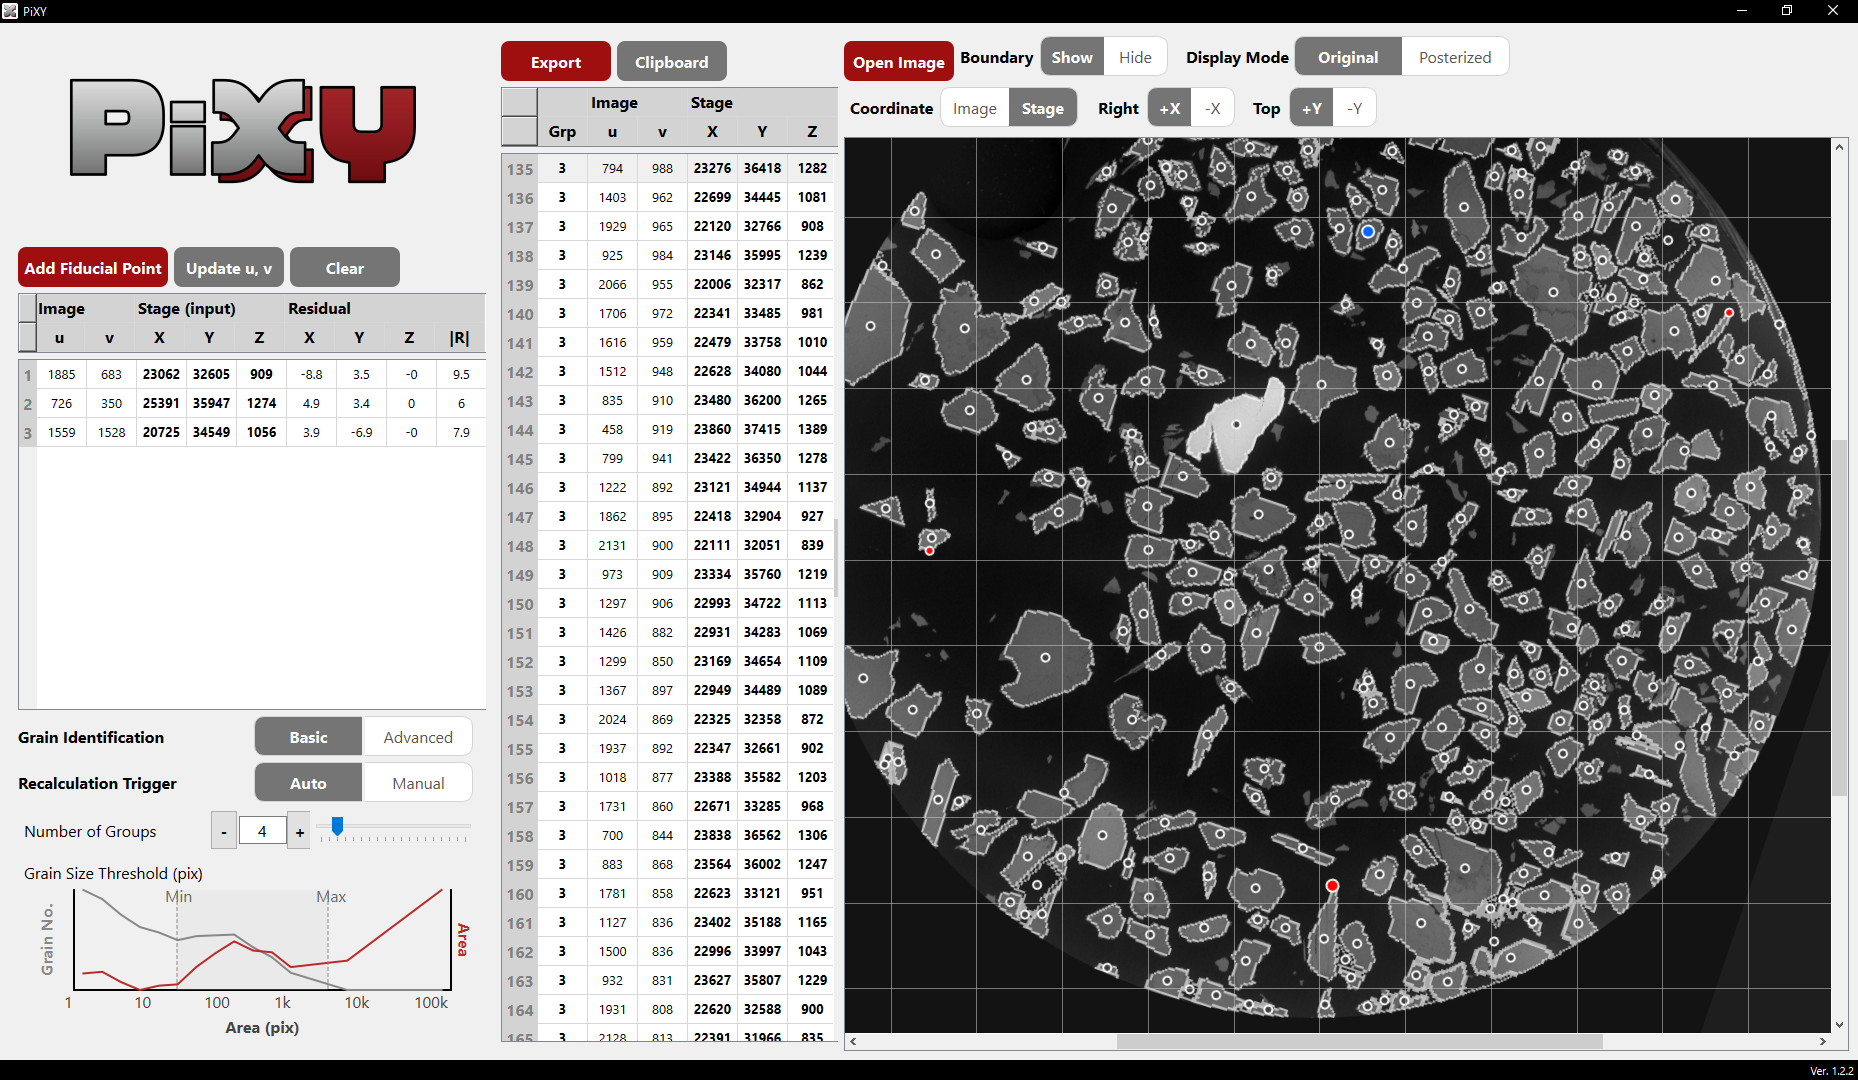
\includegraphics[width=0.8\textwidth]{documentation/images/fig_ui.png}
\caption{Example of the PiXY GUI showing overlays and parameters.}
\end{figure}
\begin{figure}[ht]
\centering
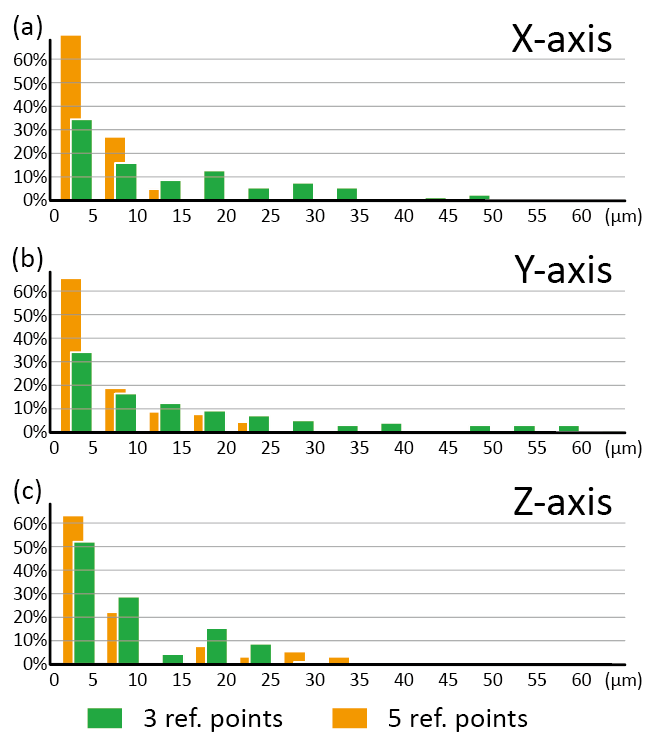
\includegraphics[width=0.8\textwidth]{documentation/images/fig_residual_hist.png}
\caption{Residual histograms comparing three vs five fiducials.}
\end{figure}
\section{Validation}
% Brief validation summary
\section{Impact and Conclusions}
\section*{Acknowledgements}
This work was supported by JSPS KAKENHI (Grant Number: 25H00682). The author acknowledges the open-source communities behind Python, OpenCV, NumPy, and PySide6.
\section*{Declaration of generative AI and AI-assisted technologies}
During the preparation of this work the author used GitHub Copilot, Google Gemini, xAI Grok, and Anthropic Claude to assist with drafting and programming tasks. The author reviewed, edited, and validated all AI-generated content and takes full responsibility for the final manuscript.
\section*{Data and software availability}
The source code is available at \url{https://github.com/YoshiakiKON/PiXY} and archived at Zenodo (DOI: 10.5281/zenodo.18174474). README includes installation and usage; detailed parameters and validation data are available in the repository's \texttt{documentation/} directory.
\end{document}
